This chapter sets out how the transfer was tested. It describes the study area and the imagery the model consumed (§3.1), the annotation protocol used to build an independent reference (§3.2), the segmentation pipeline itself (§3.3), and the accuracy measures (§3.4). It then sets out the two complementary procedures used to characterise error --- automated attribution against reference layers (§3.5) and stratified sampling with visual adjudication (§3.6) --- followed by the ablation design used to isolate the contribution of building and road subtraction (§3.7). Two checks close the chapter: one on the imagery underlying the reference and the predictions (§3.8), and one on the estimator used to correct the model's systematic bias (§3.9).

\hypertarget{study-area-and-data}{%
\section{Study area and data}\label{study-area-and-data}}

The study area is a 100 km² square centred on Leeds, divided into one hundred 1 km² cells on the British National Grid (Figure 3.1). The city centre is taken as City Square (E 429832, N 433449); cell centroids lie between 0.34 km and 7.64 km from it. Leeds was chosen as a large English city outside London with substantial surface parking in and around its core, and with complete aerial coverage at the resolution the model requires. The choice also aligns with the project's Centre for Cities framing: Leeds is among the large British cities the organisation identifies as having some of the largest density gaps relative to their international peers (Lange, Kovacevic and Johnson, 2026). A square grid rather than an administrative boundary was used so that every cell is an equal-area unit and per-cell statistics are directly comparable. The choice of areal unit is not neutral --- figures computed over zones depend on how the zones are drawn, the modifiable areal unit problem (Openshaw,
1984) --- so the unit is held constant throughout and whole-area figures are reported alongside per-cell ones.

\begin{figure}[htbp]
\centering
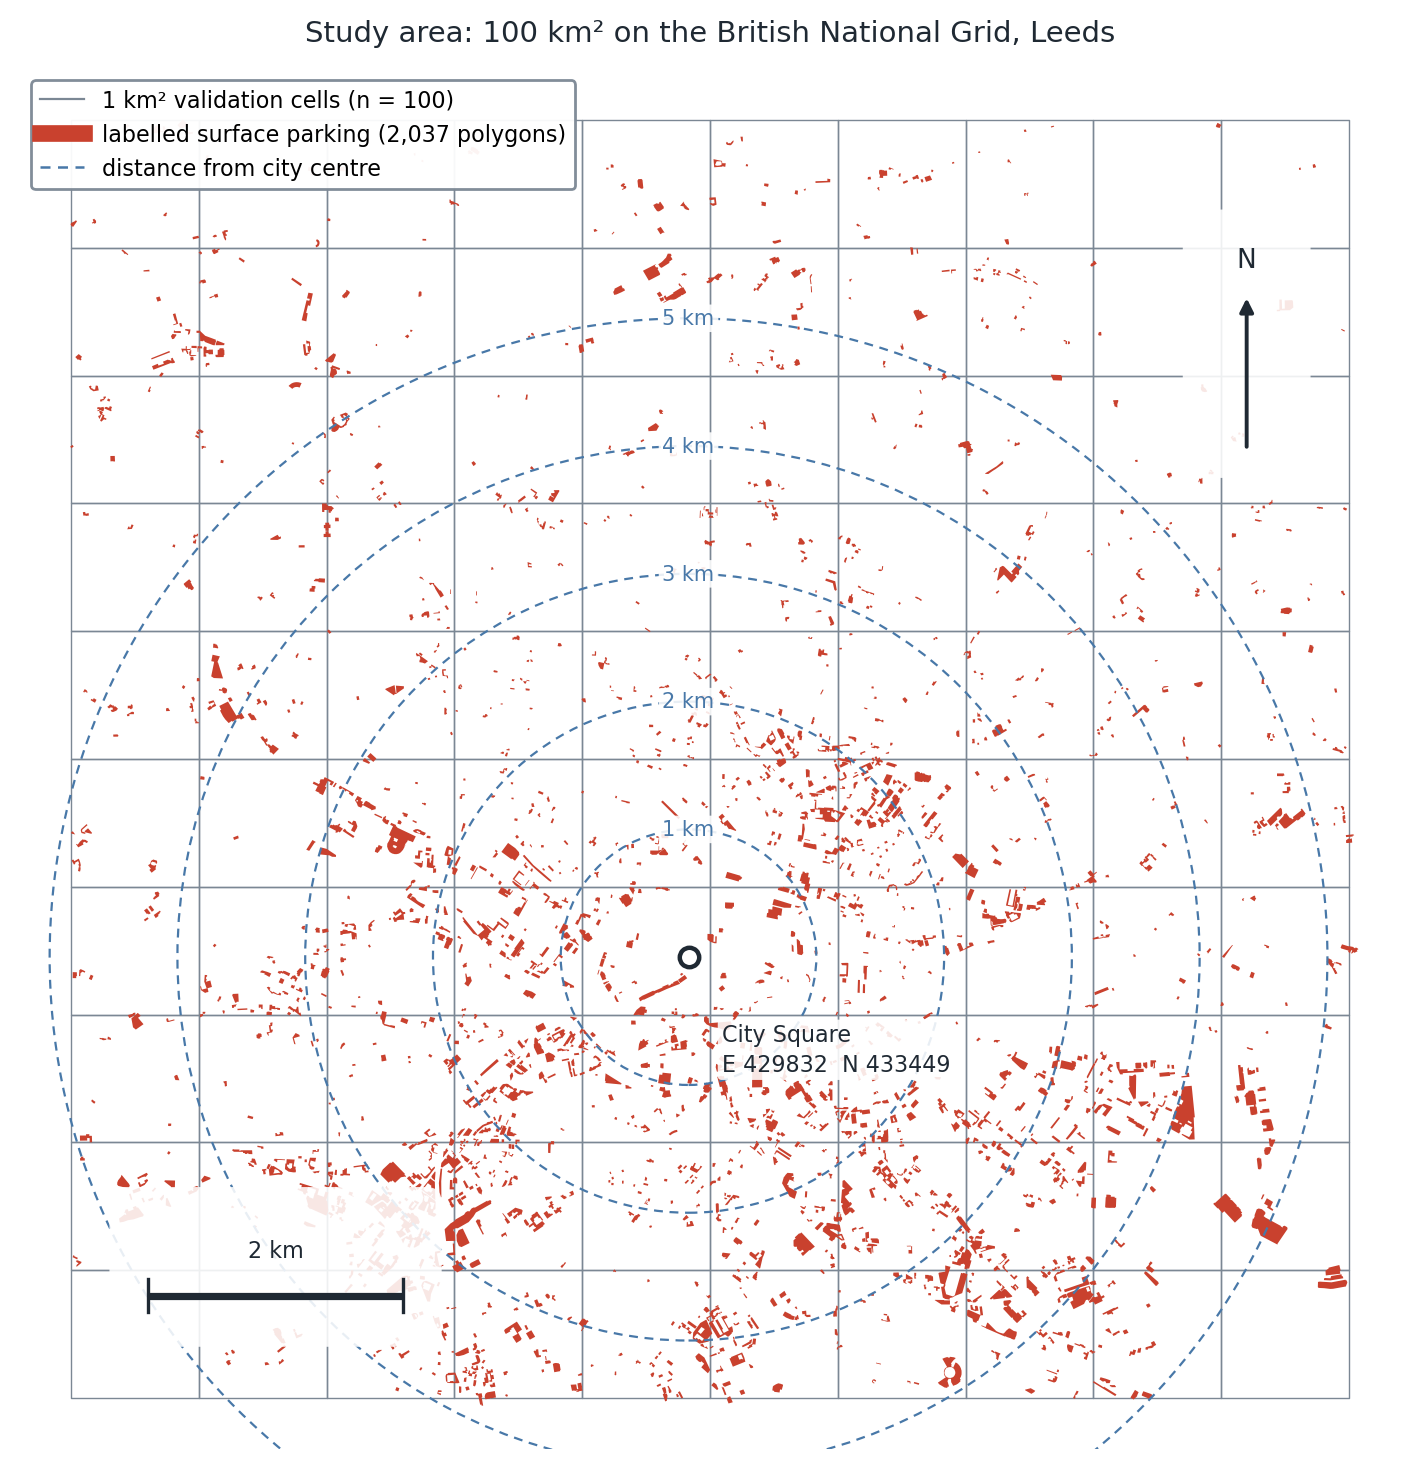
\includegraphics[width=\linewidth,height=0.82\textheight,keepaspectratio]{figures/fig_study_area.png}
\caption{The study area: one hundred 1 km² validation cells on the British National Grid, the 2,037 manually labelled surface parking polygons, and distance rings from City Square. Labelled parking is visibly concentrated in a band around, rather than at, the centre --- a pattern quantified in §4.7.}
\label{fig:3.1}
\end{figure}\restoreparskip

The imagery is Getmapping aerial photography supplied through Digimap: 100 tiles at 0.25 m ground sample distance, three visible bands (RGB), projected in EPSG:27700. All spatial operations are carried out in EPSG:27700, whose units are metres, so polygon areas are read directly in m² without further projection.

Three reference datasets are used, none of them as ground truth. OpenStreetMap building footprints and road centrelines (retrieved 25 June 2026) are inputs to the post-processing stage. OpenStreetMap land use, brownfield, pitch and \texttt{amenity=parking} polygons are used only to attribute errors after the fact. Ordnance Survey Open Greenspace supplies sports facilities. The distinction matters: reference layers are used here to explain where errors fall, and --- with the deliberate exception tested in §3.7 --- never to decide what the map should contain.

Appendix D lists the code repository, the licensing position of each dataset and the file behind every table reported here. The manual reference labels are available in the repository, but the institutionally licensed aerial imagery cannot be redistributed.

\hypertarget{annotation-protocol}{%
\section{Annotation protocol}\label{annotation-protocol}}

Accuracy figures are only meaningful against a reference that follows the definition the model was trained on. The annotation rules therefore follow those of Qiam, Devunuri and Lehe (2025), whose dataset the model was trained on, and are reproduced in full in Appendix A. The target is off-street surface parking: open-air parking surfaces visible from above, outside the public road. Labels are binary. No minimum size threshold is applied. Marked bays and the aisles connecting them are included, as is rooftop parking where the parking surface is visible from above; on-street parking and enclosed multi-storey structures are excluded. Where markings are absent, an area is labelled only where parked vehicles and a bay-and-aisle layout together make the use unambiguous. Boundaries are drawn at the edge of the paving rather than the parcel line.

One boundary inside residential parking is worth stating explicitly, because it is the commonest ambiguous case in a British city. Parking courts shared between several dwellings are labelled; driveways and forecourts serving a single household are not. A communal court resembles a small car park in layout and in what it does, while a single driveway does not. The distinction is not introduced here: UK parking measurement already separates private residential parking into driveway and communal categories, and the two were surveyed and reported separately in the London study described in §2.2 (Bates and Leibling, 2012).

Labelling was carried out in QGIS by a single annotator over a satellite basemap, producing 2,037 polygons with a confidence attribute (3 = clear, 2 = fairly clear, 1 = uncertain) and a free-text note used to flag rooftop cases. Summed individually the polygons cover 3.2677 km². Dissolving them leaves both the area and the part count unchanged, so no two labelled polygons overlap; the reference is nonetheless dissolved before every comparison, since the accuracy measures of §3.4 are only well defined on non-overlapping geometry and the property should be enforced rather than assumed. Clipping to the study grid removes 0.0081 km² where polygons cross the outer boundary, giving the 3.2597 km² used throughout. One cell (c0r9) contains no labelled parking, so recall is undefined there and per-cell statistics involving recall use \(n = 99\).

Single-annotator labelling remains a limitation, taken up in §5.5.

\hypertarget{model-and-pipeline}{%
\section{Model and pipeline}\label{model-and-pipeline}}

The model is the SegFormer (Xie et al., 2021) parking-lot segmentation network released by Qiam, Devunuri and Lehe (2025). The released checkpoint is a B5 configuration whose backbone was initialised from Cityscapes weights and fine-tuned by those authors on their parking dataset, as documented in the released model card and repository. In the primary analysis, its weights are used exactly as released: no UK imagery is used to update them. The network is therefore evaluated under zero-shot geographic transfer, although the surrounding pipeline includes the UK-specific tiling and post-processing described below and isolated by the ablation in §3.7. Appendix C reports a separate experiment on a fixed 40/10/50 cell split, comparing generic fine-tuning, positional targeted loss weighting and validation-selected thresholding on raw-pixel outputs without post-processing. Those results remain separate from the primary analysis in §§4.1--4.7.

\begin{figure}[htbp]
\centering
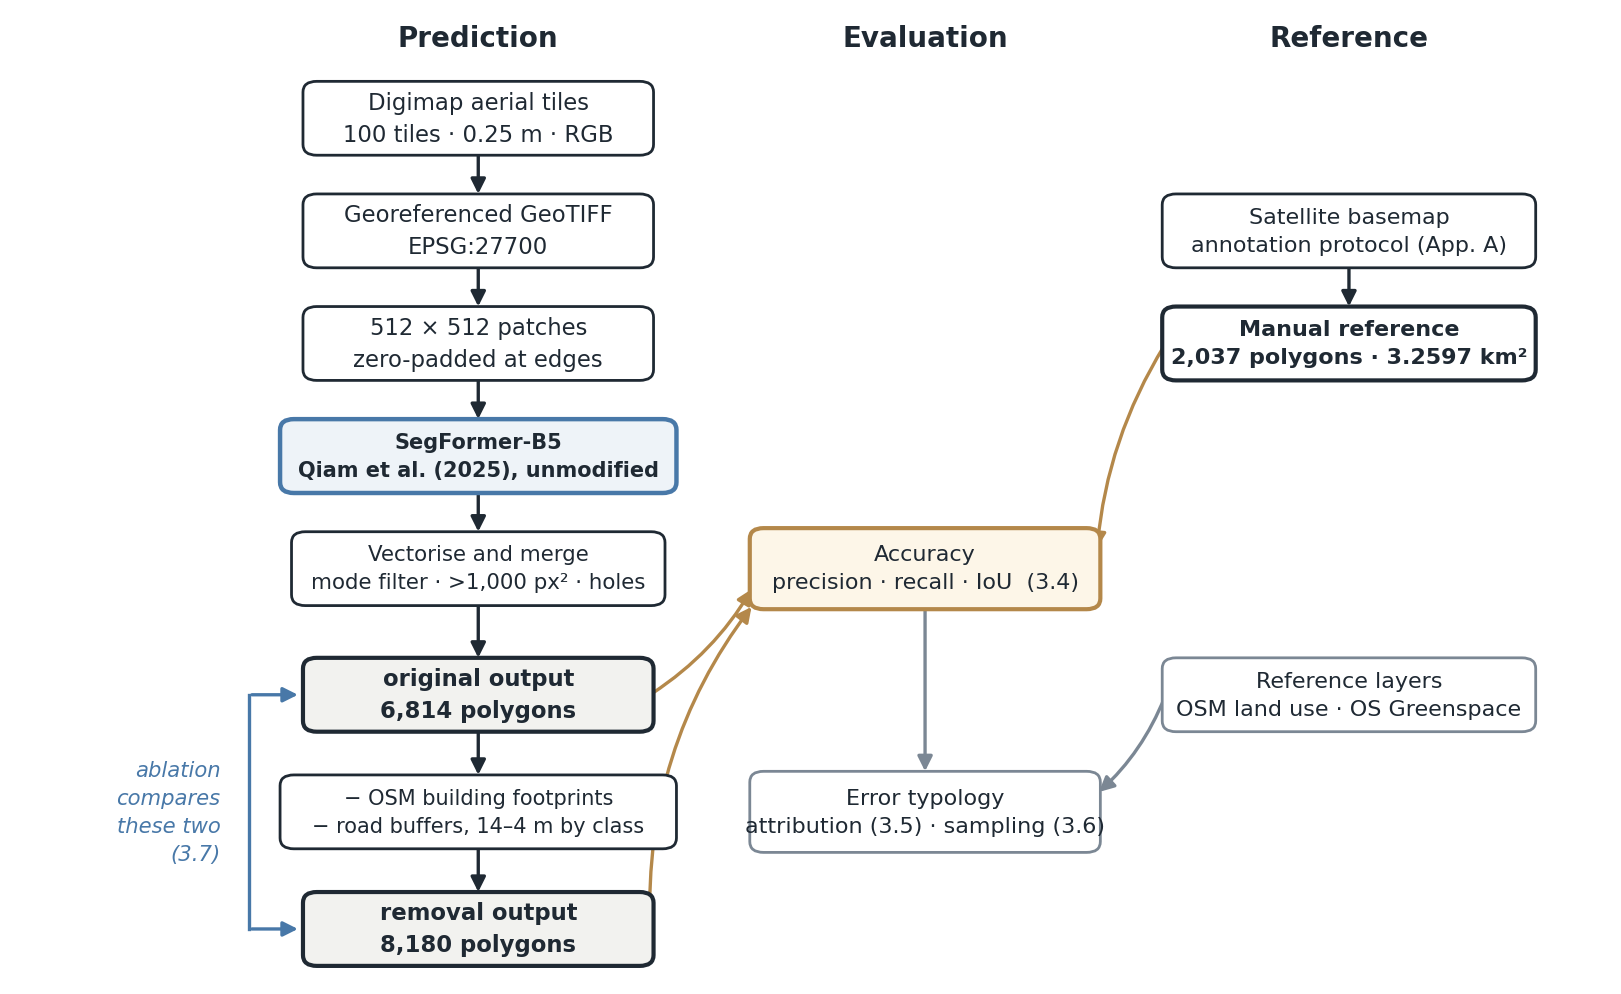
\includegraphics[width=\linewidth,height=0.82\textheight,keepaspectratio]{figures/fig_pipeline.png}
\caption{The processing chain. Prediction runs from Digimap tile to outputs before and after building and road subtraction, which the ablation of §3.7 compares. The manual reference and the model outputs meet at the accuracy measures of §3.4; the reference layers enter only at the error-attribution stage of §§3.5--3.6.}
\label{fig:3.2}
\end{figure}\restoreparskip

The pipeline proceeds in five stages. Digimap tiles and their world files are converted to georeferenced GeoTIFFs. Each tile is cut into 512 × 512 pixel patches, zero-padded at the edges. Patches are passed through the network and the upsampled logits reduced to a binary mask by argmax. Masks are cleaned with a mode filter and vectorised by contour extraction, with components below 1,000 px² (about 62 m² at 0.25 m) discarded and enclosed holes subtracted; polygons are then transformed from pixel to grid coordinates and merged across tiles.

Two post-processing subtractions follow, both UK adaptations of operations already present in the released pipeline, which likewise subtracts building footprints and buffered OpenStreetMap roads (Qiam, Devunuri and Lehe, 2025). Here, OpenStreetMap building footprints replace the source pipeline's Microsoft US building data and are subtracted under its premise that roofs are false positives --- a premise tested against rooftop parking in §3.7. Road centrelines are buffered by carriageway class (Table 3.1), rather than by recorded lane count alone, dissolved, and subtracted.

\begin{table}[htbp]
\centering
\caption{Road buffer half-widths by OSM \texttt{highway} class. Where a \texttt{lanes} tag is present, the width is the greater of the tabulated value and 3 m per lane.}\label{tab:3.1}
\begin{adjustbox}{max width=\textwidth}
\begin{tabular}{@{}lrllr@{}}
\toprule
Class & Width (m) & & Class & Width (m) \\
\midrule
motorway & 14 & & tertiary & 7 \\
trunk & 12 & & tertiary\_\allowbreak{}link & 5 \\
primary & 10 & & unclassified & 5 \\
secondary & 8 & & residential & 5 \\
motorway\_\allowbreak{}link & 9 & & living\_\allowbreak{}street & 4 \\
trunk\_\allowbreak{}link & 8 & & \emph{default} & \emph{5} \\
primary\_\allowbreak{}link & 7 & & & \\
secondary\_\allowbreak{}link & 6 & & & \\
\bottomrule
\end{tabular}
\end{adjustbox}
\end{table}
\restoreparskip

The half-widths are approximations by class rather than measured carriageway dimensions: each value is a plausible half-width for the road type the OSM class denotes, with 5 m applied to any class not listed. Footways, cycleways, bridleways, tracks, steps, pedestrian ways and service roads, among others, are excluded from the road layer, service roads in particular because they commonly run \emph{through} car parks; buffering them would remove the aisles the protocol explicitly includes. Both subtractions are evaluated rather than assumed in §3.7.

The output before subtraction (6,814 polygons) and after (8,180 polygons) are both retained. The increase in count reflects single lots being split by the subtracted geometry, which is why polygon counts are never interpreted as numbers of car parks.

\hypertarget{validation-design}{%
\section{Validation design}\label{validation-design}}

Accuracy is measured by area rather than by object, following the general practice in land-cover accuracy assessment of comparing a map against an independent reference over a defined spatial support (Foody, 2002; Olofsson et al., 2014). Let \(M\) and \(R\) denote the dissolved model and reference geometry, and \(|\cdot|\) denote area in m². Dissolving before comparison ensures overlapping geometry is not double-counted. The three quantities are then set operations:

\[
\mathrm{TP} = M \cap R, \qquad \mathrm{FP} = M \setminus R, \qquad \mathrm{FN} = R \setminus M
\]

from which

\[
\text{precision} = \frac{|\mathrm{TP}|}{|\mathrm{TP}| + |\mathrm{FP}|}, \qquad
\text{recall} = \frac{|\mathrm{TP}|}{|\mathrm{TP}| + |\mathrm{FN}|}, \qquad
\text{IoU} = \frac{|\mathrm{TP}|}{|\mathrm{TP}| + |\mathrm{FP}| + |\mathrm{FN}|}
\]

Area-based measures were chosen because the study asks how much land the map assigns to parking. Object-based matching would require an arbitrary rule for deciding whether split or merged polygons represent the same lot, particularly after post-processing. Since accuracy estimates depend on the assessment unit, the unit should reflect the intended use of the map (Stehman and Wickham, 2011; Stehman and Foody, 2019). As an internal check, \(|M| = |\mathrm{TP}| + |\mathrm{FP}|\) and \(|R| = |\mathrm{TP}| + |\mathrm{FN}|\); both hold to four decimal places.

Two aggregations over the \(n\) cells are reported. Writing \(\mathrm{TP}_c\) for the true positive area within cell \(c\), the micro (area-weighted) and macro (cell-averaged) forms of precision are

\[
p_{\text{micro}} = \frac{\sum_c |\mathrm{TP}_c|}{\sum_c\left(|\mathrm{TP}_c| + |\mathrm{FP}_c|\right)},
\qquad
p_{\text{macro}} = \frac{1}{n}\sum_c \frac{|\mathrm{TP}_c|}{|\mathrm{TP}_c| + |\mathrm{FP}_c|}
\]

and recall and IoU follow the same pattern. The terms are borrowed from classification evaluation, where the same two averages are taken over classes; here they are taken over spatial units. The micro figure treats the whole study area as one unit, so large car parks carry proportionate weight; it answers whether the \emph{total area} is right, and because summing over cells returns the whole-area quantity, it does not depend on how the cells were drawn. The macro figure weights every cell equally regardless of how much parking it contains, and does depend on it. The two are reported side by side because a global figure summarises the map as a whole while masking how accuracy varies across it, and local accuracy is better reported as an accompaniment to the global figure than in place of it (Foody, 2005; Stehman and Foody, 2019). Doing so needs a reference dense enough to support a figure in every sub-region, ordinarily the obstacle to it; here the reference is wall-to-wall rather than
sampled, so every cell carries its own. Macro is used as a diagnostic of uniformity rather than as an estimator of any population quantity, and the difference between the two is itself the result: where macro falls below micro, the model is performing worse in cells with little parking than the area-weighted figure suggests.

\hypertarget{error-typology-i-automated-attribution}{%
\section{Error typology I: automated attribution}\label{error-typology-i-automated-attribution}}

The first characterisation of error asks where FP and FN area falls relative to independent layers. It is applied exhaustively to all of it.

\textbf{Boundary effects are separated first.} Area-based measures cannot distinguish a slightly oversized car park from a false detection elsewhere when the error area is the same (Csurka, Larlus and Perronnin, 2013). Boundary IoU restores sensitivity to such errors by evaluating within a fixed contour band, particularly for large objects whose interiors dominate Mask IoU (Cheng et al., 2021). This study adapts that principle to partition, rather than rescore, boundary and non-boundary error.

FP area within a fixed distance \(d\) of a labelled lot is boundary \emph{dilation} --- the model drawing the same car park slightly too large --- as distinct from a standalone false detection elsewhere. Symmetrically, FN area within \(d\) of a predicted area is \emph{erosion}: reference area the model did not cover, but lying immediately alongside something it did find.

\[
\mathrm{FP}_{\text{dilation}}(d) = \mathrm{FP} \cap \big(R \oplus d\big), \qquad
\mathrm{FN}_{\text{erosion}}(d) = \mathrm{FN} \cap \big(M \oplus d\big)
\]

where \(\oplus\) denotes dilation by a buffer of \(d\) metres. Erosion is defined against the \emph{prediction} rather than against the reference boundary, so that it captures only reference area adjacent to a detection; defining it against the reference boundary would also count the outer edge of lots the model missed entirely, which is a detection failure rather than a boundary effect. Because no threshold separates the two cleanly, results are reported at \(d = 2\), 5 and 10 m, with 5 m used as the working value. Sensitivity to the width chosen is a known property of band-based measures rather than a peculiarity of this application (Cheng et al., 2021), which is why three are given. That 5 m is a convention rather than a natural break is also visible in the sampled evidence: the three sampled FP fragments that no category explained sit at a median distance of exactly 5.0 m from the nearest labelled lot, against 30.4--168.6 m across the substantive categories.

\textbf{Standalone FP is then attributed in two ways, reported side by side.}

\begin{itemize}
\tightlist
\item
  An exclusive partition: reference layers \(L_1,\dots,L_k\) are peeled off in sequence, each claiming only the area not already claimed, so shares sum to 100\%. Layers are ordered by how precisely they locate the phenomenon --- building footprints and sports pitches, which are exact polygons, before road proximity buffers, before broad land-use classes --- with industrial and commercial land last because it is the least specific evidence.
\item
  An unordered overlap: each layer is intersected with all FP independently, \(\mathrm{FP} \cap L_j\), so categories may overlap one another and need not sum to 100\%.
\end{itemize}

Presenting both means the substantive conclusions do not depend on the chosen ordering; as a robustness check, moving industrial land from an early position to last changes its exclusive share from 30.0\% to 29.6\%. The two have different denominators and are not differences of one another --- a point carried into the results tables, where the exclusive column includes the dilation band as its first row so that it sums to 100\%.

\textbf{FN is defined at the level of the car park, not the fragment.} An earlier version defined missed parking as reference area more than 5 m from any prediction, which conflated genuinely undetected car parks with the ragged edges of ones the model had largely found. Two diagnostics showed this: of 297 such fragments, 221 lay at a distance of exactly 5.0 m --- the threshold itself --- and 19.2\% of the area belonged to lots the model had detected to better than 70\%. FN is therefore partitioned by the \emph{coverage} of the lot it belongs to, \(\gamma = |R_i \cap M| / |R_i|\):

\begin{table}[htbp]
\centering
\begin{adjustbox}{max width=\textwidth}
\begin{tabular}{@{}lll@{}}
\toprule
Class & Coverage & Treatment \\
\midrule
whole lot missed & \(\gamma \le 0.10\) & a detection failure \\
partly detected & \(0.10 < \gamma \le 0.70\) & partial failure \\
fringe of detected lot & \(\gamma > 0.70\) & boundary imprecision \\
\bottomrule
\end{tabular}
\end{adjustbox}
\end{table}
\restoreparskip

Both cut points are conventions, as the 5 m band is, and both were varied. The lower one is not load-bearing: from \(\gamma \le 0.05\) to \(\gamma \le 0.20\) the whole-lot-missed share moves between 22.3\% and 29.9\% of FN, and the unresolved whole-lot remainder between 2.0\% and 2.9\% of labelled area, so what is concluded from it does not turn on where it sits. The upper one is more consequential --- at 0.60, 0.70 and 0.80 the fringe class takes 51.0\%, 44.4\% and 31.9\% of FN --- so that share is quoted with its threshold attached.

Only the first is treated as a detection failure, and is further attributed to subtraction-stage removal, rooftop labelling, containment within OSM buildings, or left unresolved.

Throughout, attribution is positional and is worded as such. A false positive lying on OSM industrial land is reported as \emph{located on} industrial land; it is not a claim that each such polygon was individually confirmed to be a storage yard.

\hypertarget{error-typology-ii-stratified-sampling}{%
\section{Error typology II: stratified sampling}\label{error-typology-ii-stratified-sampling}}

Automated attribution leaves a residual in each direction that no reference layer explains. These residuals are characterised by stratified random sampling with visual adjudication (Table 3.2). The design follows the three-part structure recommended for accuracy assessment --- a sampling design, a response design specifying how each sampled unit is judged, and an analysis that scales the sample back to the population (Olofsson et al., 2014; Stehman and Foody, 2019).

\begin{table}[htbp]
\centering
\caption{Sampling design. Large polygons are deliberately oversampled; the ratio estimator corrects for this.}\label{tab:3.2}
\begin{adjustbox}{max width=\textwidth}
\begin{tabular}{@{}llrrr@{}}
\toprule
Population & Stratum (m²) & Polygons & Area (km²) & Sampled \\
\midrule
Unexplained FP & 100--300 & 604 & 0.1055 & 20 \\
& 300--1,000 & 327 & 0.1656 & 25 \\
& \textgreater{} 1,000 & 61 & 0.1172 & 25 \\
Whole lots missed & 100--300 & 34 & 0.0079 & 10 \\
& 300--1,000 & 51 & 0.0292 & 15 \\
& \textgreater{} 1,000 & 17 & 0.0377 & 17 \\
OSM-only parking & 100--300 & 97 & 0.0192 & 5 \\
& 300--1,000 & 117 & 0.0625 & 10 \\
& \textgreater{} 1,000 & 59 & 0.1793 & 15 \\
\textbf{Total} & & & & \textbf{142} \\
\bottomrule
\end{tabular}
\end{adjustbox}
\end{table}
\restoreparskip

Estimates use a stratified ratio estimator (Cochran, 1977). For stratum \(h\) of known total area \(A_h\), with sample \(s_h\) and polygon areas \(a_i\), the estimated area of category \(c\) is

\[
\hat{A}_c = \sum_h A_h \cdot \frac{\sum_{i \in s_h,\, i \in c} a_i}{\sum_{i \in s_h} a_i}
\]

so that oversampling of large polygons does not distort the totals. Intervals on these estimates come from a stratified bootstrap: the inspected polygons are resampled with replacement within each stratum and the estimator recomputed 5,000 times, with each replicate's deviation scaled by \(\sqrt{1 - n_h/N_h}\) so that heavily sampled strata contribute proportionately less spread --- the largest missed-lot stratum, inspected in full at 17 of 17, contributes none. The intervals cover sampling variance only: not adjudication error, and not the frame exclusion described next.

The sampling frame excludes polygons below 100 m². For unexplained FP this removes 0.0513 km², or 11.7\% of that population (0.4396 km² in total, 0.3883 km² in frame). Percentages reported for this population are therefore shares of the frame, and the corrections derived from them (§4.6) implicitly assume the excluded slivers have the same composition as the sampled material. The assumption is conservative in the direction that matters: were the slivers composed like the sampled polygons, the upward correction to precision would be \emph{larger} than the one reported. Slivers below 100 m² are in any case more plausibly boundary artefacts than real parking, so they are not extrapolated to.

Each sample was inspected as an image chip cut from the Digimap tiles and assigned one category from a fixed list, with an optional note. Adjudication was carried out against the Digimap imagery, since a model's failure can only be assessed against the imagery it was given. Categories are organised by failure \emph{mechanism} rather than surface appearance --- what visual cue was absent --- so that the typology maps onto plausible causes rather than onto descriptions.

\hypertarget{ablation-design}{%
\section{Ablation design}\label{ablation-design}}

The contribution of each building and road subtraction is measured by a \(2 \times 2\) factorial design: the pre-subtraction prediction, buildings removed only, roads removed only, and both. Because set difference is commutative in the relevant sense,

\[
(X \setminus A) \setminus B = X \setminus (A \cup B)
\]

order does not affect this design; order matters only for the exclusive partition of §3.5. As a check that the reconstruction is faithful, applying both subtractions in one operation is compared against the pipeline's own tile-by-tile output; the two agree on all three reported measures to the displayed precision, so the ablation can be trusted to isolate these two operations.

A second set of variants tests the reference layers as filters rather than as explanations. Sports pitches, industrial and commercial land, and road buffers widened by a further 6 m are each subtracted from the finished map, singly and together. This is a deliberate test of a tempting inference: a layer that explains where errors fall might be assumed to improve the map if used to remove them. Reporting recall alongside precision for these variants is what makes the test informative.

Rooftop parking is examined separately as a case where the pipeline and the model can be shown to disagree. The sixteen labelled rooftop lots are compared against both the pre-subtraction and post-subtraction outputs.

\hypertarget{consistency-of-the-two-imagery-sources}{%
\section{Consistency of the two imagery sources}\label{consistency-of-the-two-imagery-sources}}

Labelling was carried out over a satellite basemap, whereas the model operated on Digimap aerial tiles. Differences between the sources could therefore contribute to the measured error. One spatial diagnostic and two checks of reference--imagery disagreement assess that contribution.

\textbf{(i) Spatial alignment.} For the 1,478 labelled lots larger than 300 m² and covered by the model by at least 70\%, let \(\mathbf{d}_i\) be the vector from the centroid of the labelled polygon to the centroid of the predicted area within it. A common directional displacement makes the mean vector large relative to the average displacement magnitude, whereas varying boundary errors tend to cancel. The ratio is

\[
\rho = \frac{\left\lVert \bar{\mathbf{d}} \right\rVert}{\frac{1}{n}\sum_i \lVert \mathbf{d}_i \rVert},
\qquad \bar{\mathbf{d}} = \frac{1}{n}\sum_i \mathbf{d}_i
\]

with \(\rho \to 0\) where the common directional component is small relative to the scatter, and \(\rho \to 1\) where displacement vectors share a common direction. Here \(\lVert\bar{\mathbf{d}}\rVert = 0.208\) m (0.83 pixels at 0.25 m resolution), against a mean displacement magnitude of 1.247 m (4.99 px), giving \(\rho = 0.167\). Non-zero mean components and a non-uniform direction distribution are statistically detectable (\(p < 0.001\)), but with 1,478 lots the sub-pixel magnitude is more informative than significance. This diagnostic shows no large common directional displacement among well-detected lots, so gross misregistration is unlikely to dominate the measured boundary error.

\textbf{(ii) An unresolved residual.} The whole-lot FN attribution in §3.5 leaves 0.0699 km² unresolved after separating areas associated with post-processing removal, rooftop labels and containment within building footprints. This is 2.1\% of labelled area. If the entire residual were treated as reference--imagery disagreement, recall would rise from 0.854 to 0.873. This is a sensitivity scenario for the unresolved residual, not a strict upper bound on all disagreement between the sources.

\textbf{(iii) A sampled estimate.} The stratified sample in §3.6 covers whole labelled lots with no more than 10\% coverage in both the post- and pre-subtraction outputs, excluding tagged rooftops and polygons below 100 m²; its frame contains 0.0748 km² of labelled lot area. Adjudication against the model's input imagery estimates 0.0313 km², or 1.0\% of labelled area, as not parking in that imagery. In the reference-side correction used here, removing it raises recall from 0.854 to 0.863 and leaves precision unchanged.

Separately, last-edit timestamps were retrieved for all 985 OSM parking features to test whether OSM disagreement simply reflects stale records. The 11 sampled features with no parking visible in the imagery had a median last-edit year of 2025, the most recent of any sampled category. This does not support stale OSM records as a general explanation; timestamps record any edit, including tag-only changes, rather than construction.

\hypertarget{the-calibration-estimator-and-its-spatial-grain}{%
\section{The calibration estimator and its spatial grain}\label{the-calibration-estimator-and-its-spatial-grain}}

Adjusting mapped area for commission and omission error using reference data is established practice (Olofsson et al., 2014). Here, where a map has precision \(p\) and recall \(r\), predicted area \(|M|\) relates to reference area \(|R|\) by

\[
|M| \cdot p = |\mathrm{TP}| = |R| \cdot r
\qquad\Longrightarrow\qquad
|R| = |M| \cdot \frac{p}{r}
\]

Applied to the same cells used to measure \(p\) and \(r\), this is an identity rather than an independent estimate. The factor simplifies to an area ratio:

\[
\frac{p}{r} = \frac{|\mathrm{TP}|/|M|}{|\mathrm{TP}|/|R|} = \frac{|R|}{|M|}
\]

Fitting it therefore requires only labelled and predicted total area over the calibration cells, not an object-level error analysis. Its usefulness must be tested on cells not used to fit it.

Three hold-out schemes test whether a factor fitted on one part of the city predicts another, and at what grain (Table 3.3). Each fits \(p/r\) on cells \(\mathcal{T}\) and applies it to held-out cells \(\mathcal{H}\). Whole cells, rather than polygons, are withheld because short-range spatial dependence means that randomly splitting dependent units can understate predictive error (Roberts et al., 2017). Error is reported relative to labelled area in the held-out set:

\[
e = \frac{\left(\sum_{c \in \mathcal{H}} |M_c|\right)\left(p/r\right)_{\mathcal{T}} - \sum_{c \in \mathcal{H}} |R_c|}{\sum_{c \in \mathcal{H}} |R_c|}
\]

\begin{table}[htbp]
\centering
\caption{Hold-out schemes for the calibration factor.}\label{tab:3.3}
\begin{adjustbox}{max width=\textwidth}
\begin{tabular}{@{}llrl@{}}
\toprule
Scheme & Held out & Tests & What it tests \\
\midrule
Random half split & 50 cells & 200 & transfer to a comparable area of the same city \\
Leave one distance band out & 1 band & 5 & transfer across the urban gradient \\
Leave one cell out & 1 cell & 99 & the finest grain the estimator could be used at \\
\bottomrule
\end{tabular}
\end{adjustbox}
\end{table}
\restoreparskip

Per-cell true-positive area is recovered as \(|\mathrm{TP}_c| = p_c \cdot |M_c|\) before \(p\) and \(r\) are micro-aggregated as in §3.4. Directly averaging cell precision would instead use the macro value (0.5136 rather than 0.5708) and produce a mismatched factor. The cell with no labelled parking has undefined relative error and is excluded from leave-one-out, leaving 99. Because small labelled areas destabilise relative error and inflate its mean, median absolute error in km² is also reported.
